\subsection{Big Data}
\subsubsection{Contexto Histórico}
Al igual que todos los términos que surgen a partir de avances tecnológicos, no existe un consenso claro de cómo definir \textit{Big Data}. \cite{manyika2011big} definen este concepto como los conjuntos de datos cuyo tamaño está más allá de la habilidad de las herramientas software de base de datos para capturar, almacenar, gestionar y analizar. Nótese que esta definición no hace referencia a un tamaño mínimo del conjunto de datos, sino que asume que la tecnología avanza constantemente (como así también las herramientas), por lo cual, la definición se ``mueve'' con el tiempo. Por otro lado, también es interesante tomar otra arista en la definición de este concepto: la consultora Gartner en su sitio web\footnote{Concepto de Big Data en el glosario de Gartner: \url{https://www.gartner.com/en/information-technology/glossary/big-data}. Último acceso: Febrero 2021.} lo define como ``Big Data son activos de información caracterizados por su alto volumen, velocidad y variedad que demandan formas innovadoras y rentables de procesamiento de información para mejorar la compresión y la toma de decisiones'', haciendo énfasis en la multiplicidad de características del concepto de Big Data.

\bigskip El comienzo de sobrecarga de información, recientemente mencionado, data del año 1880, cuando el censo de los Estados Unidos tarda 8 años en tabularse. Ante esta situación Herman Hollerith inventó la máquina tabuladora eléctrica basada en tarjetas perforadas\footnote{Herman Hollerith, US Census Boureau: \url{https://www.census.gov/history/www/census_then_now/notable_alumni/herman_hollerith.html}. Último acceso: Febrero 2021.}. El censo en 1890 fue un éxito rotundo e, incluso, la máquina diseñada fue utilizada para los censos de Canadá, Noruega y Austria al año siguiente. En el año 1941, los científicos empiezan a utilizar el término “explosión de la información”, que fuera citado en el periódico The Lawton Constitution\footnote{The Lawton Constitution: \url{http://www.swoknews.com/}.  Último acceso: Febrero 2021.}, haciendo alusión a la dificultad de administrar toda la información disponible. Gradualmente, se identificaron avances concretos en materia de procesamiento de datos y criptografía, motivados particularmente por los sucesos bélicos de la época. Un ejemplo es el dispositivo llamado Colossus \citep{copeland2004colossus} que buscaba e interceptaba mensajes a una tasa de miles de caracteres por segundo. Unos años más tarde, en 1951, el concepto de \textit{memoria virtual} es introducido por el físico alemán Fritz-Rudolf Güntsch, como una idea que trataba el almacenamiento finito como infinito.

\bigskip A partir de la década del 80’, los avances tecnológicos, especialmente en sistemas MRP (planificación de recursos de fabricación), permitieron nuevas formas de organizar, almacenar y generar datos. En este sentido, IBM se destaca y define una arquitectura para los informes y análisis de negocio (EBIS)\footnote{Acrónimo para EMEA (Europe, Middle East and Africa) Business Information System.}, que se convierte en la base del almacenamiento de datos en forma centralizada para usuarios finales \citep{devlin1988architecture}; es decir, el \textit{data warehousing}. Hacia finales de los 80’, Tim Berners-Lee, inventa la \textit{World Wide Web} \citep{berners1992world}, invento que provocaría el impacto más grande hasta la actualidad con respecto a la generación, identificación, almacenamiento y análisis de grandes volúmenes de datos de diversa naturaleza.

\bigskip El inicio de los años 90’ marcan un antes y un después en lo relativo al tratamiento y almacenamiento de datos. El crecimiento tecnológico fue explosivo, tal es así que el almacenamiento digital empieza a ser más conveniente y rentable que el papel para almacenar datos \citep{morris2003evolution}. Es en 1990 cuando surgen las plataformas de \textit{Business Intelligence} (BI) y los rediseños de software al estilo \textit{Enterprise Resource Planning} (ERP). En este contexto, \cite{cox1997application} afirman que el crecimiento de la cantidad de datos que debe manejar un sistema de información empieza a ser un problema en materia de almacenamiento y visualización de los datos, situación que denominaron como “el problema del Big Data”. Así, 1997 es un año clave, en el que se realizan un gran porcentaje de estudios y publicaciones que se enfocan en averiguar cuánta información hay disponible a nivel mundial y su crecimiento\footnote{Michael Lesk publica \textit{“How much information is there in the world?”} (1997): \url{http://www.lesk.com/mlesk/ksg97/ksg.html}. Último acceso: Febrero 2021.} y, en consecuencia, se estima que el crecimiento de Internet es aproximadamente del 100\% anual, y que superaría al tráfico de voz para el año 2002 \citep{coffman1998size}.

\bigskip En el año 2001, se introduce el concepto de \textit{Las 3 V’s: Volumen, Velocidad y Variabilidad de los datos} \citep{laney20013d}, fundantes sobre la temática y que sería mundialmente aceptado una década más tarde. Por otro lado, también en 2001, aparece el concepto de \textit{Software como un Servicio} (SaaS) \citep{hoch2001software}, un modelo disruptivo de servicios centralizados y acceso a los mismos mediante clientes finos (típicamente exploradores web), dando la posibilidad del escalamiento horizontal de sistemas de información y la generación de estándares de comunicación. Esta situación provocó que empresas como Oracle\footnote{Oracle: \url{https://www.oracle.com}. Último acceso: Febrero 2021.}, SAP\footnote{SAP: \url{https://www.sap.com}. Último acceso: Febrero 2021.} y Peoplesoft\footnote{Peoplesoft: adquirida por Oracle en Enero de 2005.} empiecen a centrarse en el uso de servicios web, permitiendo así la generación de datos en forma masiva por usuarios finales. Así, en 2006, nace Apache Hadoop\footnote{Apache Hadoop: http://hadoop.apache.org/. Último acceso: Febrero 2021.}, una solución de código abierto que permite el procesamiento en paralelo y distribuido de enormes cantidades de datos en forma escalable. Posteriormente, en 2008, se empieza a pensar al Big Data como la mayor innovación en informática en la última década, ya que ha transformado la forma en que los motores de búsqueda acceden a la información, las actividades de las compañías, las investigaciones científicas, la medicina, y las operaciones de defensa e inteligencia de los países, entre otras tantas actividades. Más aún, se ha comenzado a ver su potencial para recopilar y organizar datos en todos los ámbitos de la vida cotidiana \citep{bryant2008big}, tales como redes sociales, estadísticas deportivas, o avances médicos y genéticos.

\subsubsection{Map-Reduce}
Map-reduce es un modelo de programación popular para el procesamiento de grandes cantidades de datos mediante computación distribuida \citep{condie2010mapreduce}.  En pocas palabras, se especifica una función \textit{map} que procesa pares clave-valor para generar un conjunto de pares clave-valor intermedios, y una función \textit{reduce} que combina todos los valores intermedios asociados con la misma clave \citep{dean2008mapreduce}. En lenguajes de programación funcionales así como también lenguajes de alto nivel modernos, es posible escribir expresiones de estilo \textit{lambda}\footnote{Las funciones Lambda no tienen definido un identificador. Son también conocidas como funciones anónimas.}, en las cuales es posible paralelizar y ejecutar programas en clusters distribuidos sin la necesidad de tener en cuenta los detalles de partición de datos y subprocesamiento.

\paragraph{Arquitectura Hadoop}
La librería de software Apache Hadoop es un framework que posibilita el procesamiento de grandes conjuntos de datos entre clusters de computadoras usando modelos de programación simples. Para posibilitar esto, Hadoop se basa en una arquitectura de archivos propia, llamada HDFS\footnote{Siglas en inglés para Hadoop Distributed File System.} (Sistema de Archivos Distribuido Hadoop). En la mayoría de los procesos basados en Hadoop, HDFS es utilizado para almacenar la entrada del paso ``map'' y la salida del paso ``reduce'', pero no los resultados intermedios, ya que ellos se almacenan en el sistema de archivo de cada uno de los nodos \citep{condie2010mapreduce}. Según el sitio oficial\footnote{Arquitectura HDFS: https://hadoop.apache.org/docs/stable/hadoop-project-dist/hadoop-hdfs/HdfsDesign.html. Último acceso: Febrero 2021.}, HSFS es altamente tolerante a fallos y es diseñado para ser ejecutado en computadoras de bajo costo. Además, HDFS provee gran productividad accediendo a los datos de una aplicación y es posible usarlo en grandes conjuntos de datos.

\bigskip HDFS tiene una arquitectura maestro-nodo\footnote{Del inglés, master-node architecture.}. Un cluster HDFS (conjunto de nodos maestro-nodos) consiste en un \textit{NameNode}, que es un servidor maestro que maneja el espacio de nombres del sistema de archivos y regula el acceso a archivos. Además, hay un número de \textit{DataNodes}, usualmente uno por cada nodo en el cluster, que maneja el almacenamiento de datos en archivos. Internamente, un archivo es dividido en uno o más bloques, y esos bloques son almacenados en DataNodes. Por otro lado, el NameNode ejecuta operaciones tales como abrir, cerrar, y renombrar archivos y directorios.
\bigskip
\begin{figure}[h!]
	\centering
	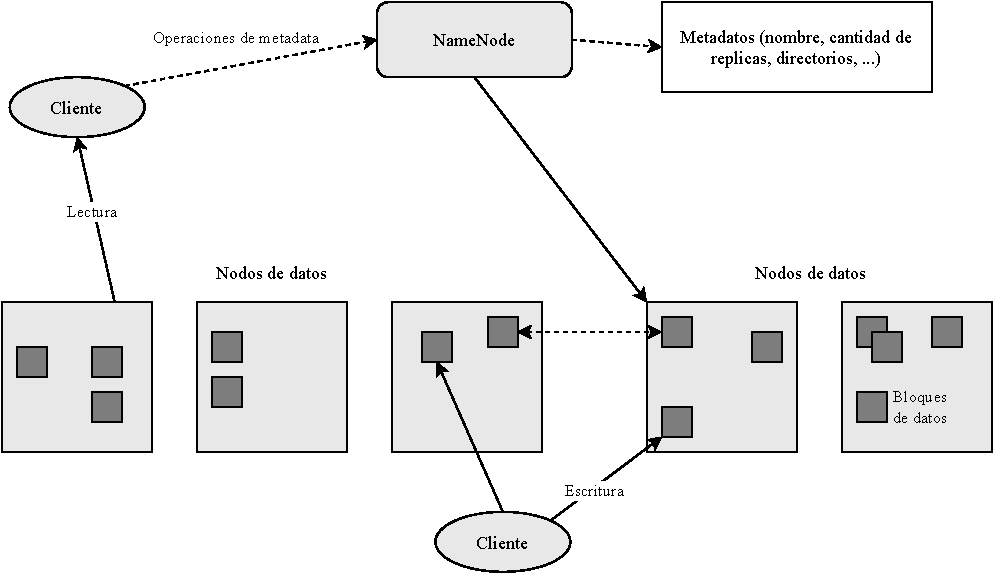
\includegraphics[width=0.9\linewidth]{7_marco_teorico/imagenes/arquitectura_hdfs}
	\caption{Arquitectura HDFS.}
	\label{fig:arquitectura_hdfs}
\end{figure}

\bigskip Tanto el NameNode como el DataNode son piezas de software diseñadas para correr, típicamente, en sistemas operativos GNU/Linux. Además, como HDFS está construido utilizando el lenguaje de programación Java, puede ser desplegado en un rango amplio de máquinas. La Figura \ref{fig:arquitectura_hdfs} muestra como un programa cliente interactúa con los nodos de datos para escritura y lectura, mientras que también interactúa con el NameNode para realizar operaciones de metadata.

\paragraph{Apache Spark}
Apache Spark es una plataforma de código abierto escrita en Scala\footnote{Sitio oficial del lenguaje de programación Scala: https://www.scala-lang.org/. Último acceso: Febrero 2021.}, para procesamiento de datos a gran escala y preparado para tareas de Machine Learning iterativas \citep{meng2016mllib}. En alto nivel, una aplicación Spark consiste en un programa “driver” que ejecuta la función “main” y varias operaciones en paralelo en un cluster de computadoras\footnote{Red de computadoras de alta velocidad que se comportan como si fuesen un único servidor. No confundir con la definición de “cluster” en algoritmos de clustering.}.

\bigskip El paralelismo en un cluster de computadoras realizado por Spark se basa en particiones de datos, por ejemplo, si se desea procesar un conjunto de datos de un millón de registros y se cuenta con un cluster de 4 nodos (sin contar el nodo principal), cada uno de ellos procesará 250.000 registros. Para conseguir esto de una forma que pueda ser entendible para un desarrollador, la plataforma cuenta con una abstracción de datos llamada RDD o \textit{Resilient Distributed Dataset} (o conjunto de datos distribuido resiliente), la cual es una colección de datos particionados a través de los nodos de cluster que pueden operar en paralelo. Los RDDs son creados desde un archivo HDFS o una colección Scala existente en el programa driver. También es posible almacenarlos en memoria, permitiendo que estas colecciones sean reusadas eficientemente entre operaciones paralelas.

\bigskip Los RDDs permiten dos tipos de operaciones: \textit{transformaciones}, las cuales crean un conjunto de datos desde uno existente, y \textit{acciones} u \textit{operaciones terminales}, que devuelven un valor al programa driver luego de ejecutar una cierta cantidad de cómputos en el conjunto de datos. Estas operaciones se condicen con el modelo de programación map-reduce en el cual se basa Hadoop. Por ejemplo, map es una transformación que opera en cada uno de los elementos del conjunto de datos y devuelve un nuevo RDD representando los resultados. Por otro lado, reduce es una operación que agrega todos los elementos de un conjunto de datos usando alguna función y devolviendo un resultado final.

\bigskip Todas las transformaciones son \textit{lazy}, esto es, secuencias de acciones imperativas las cuales son retrasadas hasta que el resultado es requerido \citep{launchbury1993lazy}, es decir, las transformaciones aplicadas a un conjunto de datos son recordadas hasta que es necesario devolver un resultado final al programa driver. Además, es posible almacenar un RDD en memoria (o disco rígido) logrando así mantener elementos disponibles en un cluster para un acceso rápido en caso de que una transformación sea requerida más de una vez.